\section{Relations de comparaison}

%------------------------------------------------
\begin{frame}
\frametitle{Fonctions dominées}

\begin{definition}
Soit $f : I \rightarrow \mathbb{R}$ et $\varphi : I \rightarrow \mathbb{R}$ et $a \in I$. 
 Alors $f$ est \textbf{dominée} par $\varphi$ au voisinage de $a$, s'il existe une fonction $u : I \rightarrow \mathbb{R}$ bornée au voisinage de $a$ et telle que $f = \varphi u$ au voisinage de $a$. 
 On note
 \begin{equation*}
     f = \mathcal{O}(\varphi)
 \end{equation*} 
\end{definition}
\invisible<1>{
\vspace*{0.3 cm}
\textcolor{cadmiumgreen}{\textbf{Exemple} : } 
$f(x) = x^2 \sin \left(\dps \frac{1}{x} \right)$  sur $\ \mathbb{R}$ et $\varphi(x) = x^2$.
Alors
\begin{equation*}
    f(x) = \varphi(x) \textcolor{red}{u}(x) \quad \text{avec} \quad \textcolor{red}{u}(x) = \sin \left(\frac{1}{x} \right). 
\end{equation*}
Or \alert{$u$ est bornée} donc $f = \mathcal{O}(\varphi)$.
 \invisible<2>{
 }}
\end{frame}
%%%%%
\begin{frame}
\frametitle{Fonctions négligeables}
\vspace{-0.1 cm}
\begin{definition}
on dit que $f$ est \textbf{négligeable} devant $\varphi$ au voisinage de $a$, s'il existe une fonction $\varepsilon$ définie sur $I$ tel que $f = \varphi \varepsilon$ au voisinage de $a$ et $\lim_{\substack{a}} \varepsilon = 0$. On note $f = o(\varphi)$.
  \end{definition}
  \invisible<1>{
  \textcolor{cadmiumgreen}{\textbf{Exemple :}}
  $x^3 = o(x^2)$ au voisinage de $0$ car $x^3 = \textcolor{red}{x} \times x^2$ avec $\textcolor{red}{\varepsilon}(x) = x$ et $\dps \lim_{x \rightarrow 0} \textcolor{red}{\varepsilon}(x) = 0$.
  \begin{figure}[h]
    \centering
    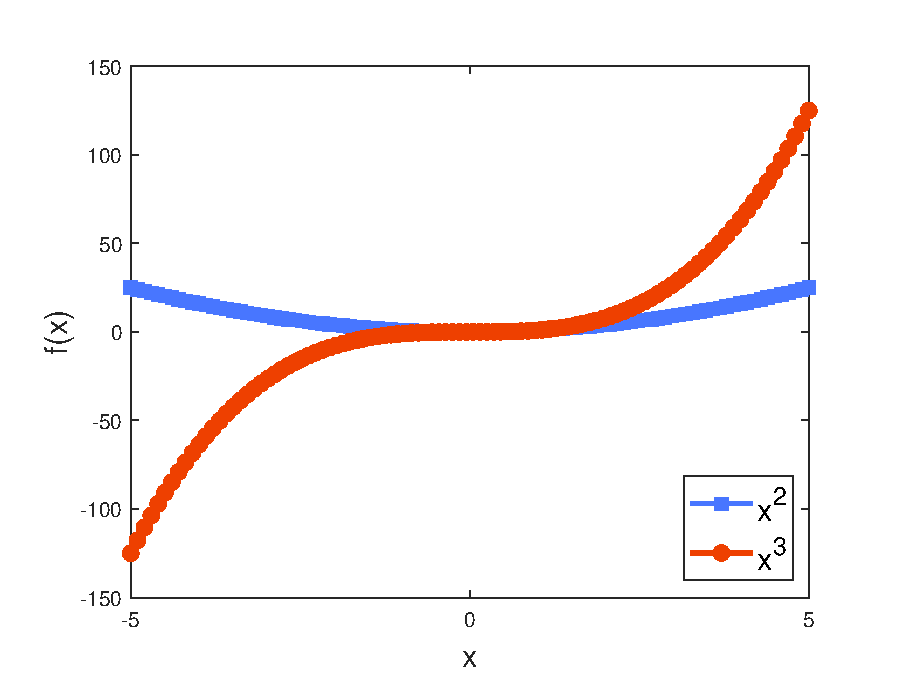
\includegraphics[scale = 0.35]{fig_x2_x3}
\quad
    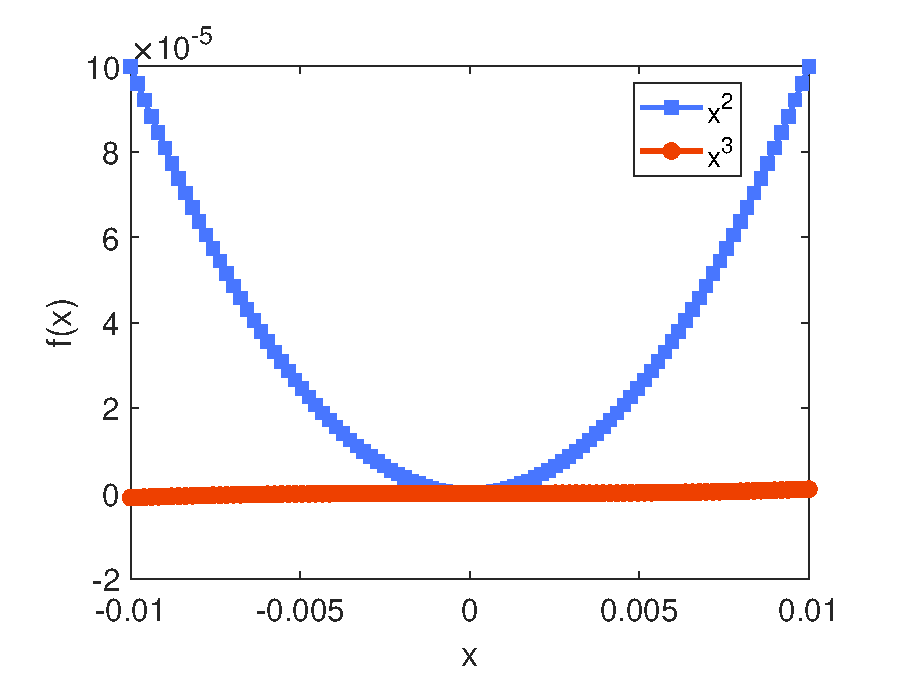
\includegraphics[scale = 0.35]{fig_x2_x3_zoom}
  \end{figure}
  \invisible<2>{
  }}
\end{frame}

%------------------------------------------------
\begin{frame}
	\frametitle{Quelques résultats}
		\begin{proposition}
Soit $f : I \rightarrow \mathbb{R}$ une fonction et $a \in I$.
\vspace{0.2 cm}
   \begin{enumerate}
   \item
     La fonction $f$ est bornée au voisinage de $a$ si, et seulement si $f = \mathcal{O}(1)$.
\vspace{0.3 cm}
   \item
     La fonction $f$ tend vers $0$ en $a$ si, et seulement si $f= o(1)$.
     \end{enumerate}
\end{proposition}
\vspace{0.2 cm}
\invisible<1>{
\textbf{Démonstration :}
\invisible<2>{
}}
\vspace{0.2 cm}
  \begin{enumerate}
  \item
 \invisible<1>{
 $\alert{(\Rightarrow)}$
On suppose $f$ bornée au voisinage de $a$. 
$\forall x \in \textcolor{cadmiumgreen}{\mathcal{V}_{a}}$, $|f(x)| = f(x) \times \underbrace{\textcolor{darkmagenta}{1}}_{\text{bornée}}$. 
    Donc $f = \mathcal{O}(1)$.
    \\
    \invisible<2>{
  \vspace{0.2 cm}
   $\alert{(\Leftarrow)}$  $f = \mathcal{O}(1)$. 
   Alors $\exists \varphi$  bornée sur $\textcolor{cadmiumgreen}{\mathcal{V}_{a}}$ tel que $f = \varphi \times 1$ sur $\textcolor{cadmiumgreen}{\mathcal{V}_{a}}$. 
Donc $f$ bornée sur $\textcolor{cadmiumgreen}{\mathcal{V}_{a}}$.
\invisible<3>{
}}}
\end{enumerate}
\end{frame}
%------------
\begin{frame}
\begin{enumerate}\setcounter{enumi}{1}
  \item
$\alert{(\Rightarrow)}$  $f$ tend vers $0$ en $a$ :
\begin{equation*}
\forall \varepsilon > 0 \ \exists \textcolor{cadmiumgreen}{\eta_1} > 0 \ \forall x \in ]a - \textcolor{cadmiumgreen}{\eta_1}, a + \textcolor{cadmiumgreen}{\eta_1}[, \ |f(x)|  \leq \varepsilon.    
\end{equation*}
On pose
\begin{equation*}
\begin{array}{ccccc}
\varphi & : & \mathcal{D}_f & \to & \mathbb{R} \\
 & & x & \mapsto & f(x) \\
\end{array}
\qquad \lim_{x \rightarrow a} \varphi(x) = 0
\end{equation*}
    Alors  
 $f = o(1)$.
\\
\vspace{0.4 cm}
\invisible<1>{
$\alert{(\Leftarrow)}$  $f=o(1)$ au voisinage de $a$. 
\vspace*{0.2 cm}
Alors  $\exists \textcolor{darkmagenta}{\varphi}$ définie au voisinage de $a$ tel que $f = \textcolor{darkmagenta}{\varphi} 1$ au voisinage de $a$ avec $\lim_{a} \varphi = 0$. 

Or $\lim_{a} \varphi \in \mathcal{V}_a$ donc $\lim_{a} f = \lim_{a} \varphi = 0$.
\invisible<2>{
}}
    \end{enumerate}
\end{frame}
%------------------------------------------------

\begin{frame}{Quelques remarques}
\begin{enumerate}
    \item <1->
Lorsque $f = o(g)$ au voisinage de $a \in I$, $f = g \times \varepsilon$ au voisinage de $a$ et $\lim_{a} \varepsilon = 0$. Mais, $\lim_{a} \varepsilon \not \rightarrow 0$ sur $I$ tout entier.
\\
\vspace{0.2 cm}
  \textcolor{cadmiumgreen}{\textbf{Contre exemple :}} 
  \begin{equation*}
      f : x \mapsto x^3 \quad \text{et} \quad g : x \mapsto x^2 \quad \text{sur} \ \mathbb{R}.
  \end{equation*}
  On a $f=o(g)$ au voisinage de $0$ (\textcolor{darkmagenta}{$\varepsilon(x) = x$}) mais $\varepsilon(x) \neq 0 \ \forall x \in \mathbb{R}^{*}$.  
\\
\vspace{0.2 cm}
 \item <2->
  Si $f=o(h)$ et $g=o(h)$ au voisinage de $a$ alors $f$ n'est pas forcément égal à $g$. 
  \\
\vspace{0.2 cm}
  \textcolor{cadmiumgreen}{\textbf{Contre exemple :}}
  \begin{equation*}
   f : x \mapsto x^3 \quad    g : x \mapsto x^4 \quad h : x \mapsto x^2.
  \end{equation*}
  On a $f=o(h)$ au voisinage de $0$ et $g=o(h)$ au voisinage de $0$ mais $f \neq g$.
\vspace{0.3 cm}
    \item <3->
  Le même phénomène s'observe pour la notation $\mathcal{O}$.
\end{enumerate}
      
\end{frame}
%%--------------------
\begin{frame}{Règles de calcul}

\begin{proposition}
    \begin{enumerate}
  \item
  $f = o(\varphi) \Rightarrow f = \mathcal{O}(\varphi) \qquad  $ \textcolor{midnightblue}{(négligeable $\Rightarrow$ bornée)}
  \vspace{0.3 cm}
  \item
$f_1 = \mathcal{O}(\varphi)$ et $f_2 = \mathcal{O}(\varphi)$ $\Rightarrow f_1 + f_2 = \mathcal{O}(\varphi)$ \quad  \textcolor{midnightblue}{\small{(somme de fonctions bornée est bornée)}}
\vspace{0.3 cm}
\item
$f_1 = \mathcal{O}(\varphi_1)$ et $f_2 = \mathcal{O}(\varphi_2)$ $\Rightarrow f_1 f_2 = \mathcal{O}(\varphi_1 \varphi_2)$ 
\vspace{0.3 cm}
\item
$f_1 = o(\varphi)$ et $f_2 = o(\varphi)$ $\Rightarrow f_1  + f_2 = o(\varphi)$ \quad \textcolor{midnightblue}{\small{(somme de termes négligeable est négligeable)}}
\vspace{0.3 cm}
\item
$f_1 = o(\varphi_1)$ et $f_2 = o(\varphi_2)$ $\Rightarrow f_1 f_2 = o(\varphi_1 \varphi_2)$
\vspace{0.3 cm}
\item
$f = \mathcal{O}(\varphi_1)$ et $\varphi_1 = \mathcal{O}(\varphi_2)$ $\Rightarrow f = \mathcal{O}(\varphi_2)$ \quad \textcolor{midnightblue}{\small{(transitivité de la domination)}}
\vspace{0.3 cm}
\item
$f = o(\varphi_1)$ et $\varphi_1 = o(\varphi_2)$ $\Rightarrow f = o(\varphi_2)$ \textcolor{midnightblue}{\small{(transitivité de la négligence)}}
  \end{enumerate}
  \end{proposition}
\end{frame}
%------------
\begin{frame}{Démonstration}
\begin{enumerate}
        \item <1-> 
    $f = o(\varphi)$ au voisinage d'un point $a$ $\Rightarrow \ f = g \varphi$ au voisinage de $a$ et \textcolor{darkmagenta}{$\lim_{a} g = 0$}. 
%Ce qui s'écrit aussi à l'aide de la définition de la limite
\begin{equation*}
\textcolor{darkmagenta}{\forall \varepsilon > 0 \ \exists \eta > 0 \ \forall x \in  ]a-\eta, a+\eta[, \ |g(x)| \leq \varepsilon.}
\end{equation*}
La fonction $g$ est donc bornée au voisinage de $a$.
Alors $f = \mathcal{O}(\varphi)$.

\item <2->
  \invisible<1>{
    $f_1 = \mathcal{O}(\varphi)$ alors $f_1 = \varphi u$ au voisinage de $a$ où $u$ est bornée au voisinage de $a$.
  \begin{equation*}
    \exists \eta_1 > 0 \ \forall x \in ]a - \eta_1, a + \eta_1[, \ f_1(x) = \varphi(x) u(x).
  \end{equation*}
  \invisible<2>{
    $f_2 = \mathcal{O}(\varphi)$ donc $f_2 = \varphi v$ au voisinage de $a$.
\begin{equation*}
 \exists \eta_2 > 0 \ \forall x \in ]a - \eta_2, a + \eta_2[, \ f_2(x) = \varphi(x) v(x).
\end{equation*}
\invisible<3>{
Pour \textcolor{darkmagenta}{$\eta = \min(\eta_1, \eta_2)$} on a $\forall x \in ]a - \textcolor{darkmagenta}{\eta}, a + \textcolor{darkmagenta}{\eta} [ \ (f_1+ f_2)(x) = \varphi(x) (u + v)(x)$. 
  Comme $u+v$ bornée au voisinage de $a$ on a $f_1 + f_2 = \mathcal{O}(\varphi)$.
  \invisible<4>{
  }}}}
\end{enumerate}
    
\end{frame}
%--------
\begin{frame}
\frametitle{Démonstration}
    \begin{enumerate}\setcounter{enumi}{3}
    \item 
      \begin{itemize}
      \item
        $f_1 = o(\varphi)$ au voisinage de $a$ alors il existe une fonction $\varepsilon_1$ définie au voisinage de $a$ tel que
        \begin{equation*}
\lim_{x \rightarrow a} \varepsilon_1(x) = 0 
        \end{equation*}
        et vérifiant $f_1 = \varepsilon_1 \varphi$ au voisinage de $a$
        \vspace*{0.3 cm}
      \item
$f_2 = o(\varphi)$ au voisinage de $a$ alors il existe une fonction $\varepsilon_2$ définie au voisinage de $a$ tel que 
\begin{equation*}
 \lim_{x \rightarrow a} \varepsilon_2(x) = 0
\end{equation*}
vérifiant $f_2 = \varepsilon_2 \varphi$ au voisinage de $a$.
%\\
        \end{itemize}
        
\vspace{0.3 cm}
Ainsi, la fonction $\varepsilon = \varepsilon_1 + \varepsilon_2$ est bien définie au voisinage de $a$ et $\lim_{x \rightarrow a} \varepsilon (x) = 0$. 
Alors, $f_1 + f_2 = o(\varphi)$.
    \end{enumerate}
\end{frame}
%-----------
\begin{frame}{Règle pratique}
      \begin{proposition}
    Soit $I$ un intervalle de $\mathbb{R}$ et $a \in I$.
Supposons que $\varphi$ ne s'annule pas sur $I \backslash{a}$.
Alors au voisinage de $a$
\vspace{0.3 cm}
\begin{enumerate}
\item $f$ est dominée par $\varphi$ si, et seulement si,  $\dps \frac{f}{\varphi}$ est bornée au voisinage de $a$.
\item
$f$ est négligeable devant $\varphi$ si, et seulement si, $\lim_{x \rightarrow a} \dps \frac{f(x)}{\varphi(x)} = 0$.
\end{enumerate}
\end{proposition}
\end{frame}
%%-----------
\begin{frame}{Fonctions équivalentes}
    \begin{definition}
Soient $f$ et $g$ définies sur un intervalle $I$. On dit que $f$ est équivalente à $g$ au voisinage de $a$, s'il existe une fonction $h$ définie sur $I$ telle que $f=gh$ au voisinage de $a$ et $\lim_{x \rightarrow a} h(x) = 1$. On note $f \underset{a}{\sim}  g$.
\end{definition}
\invisible<1>{
\textcolor{cadmiumgreen}{\textbf{Exercice :}}
Soient $f$ et $g$ deux fonctions définies sur $\mathbb{R}$ par
  $f(x) = \sin(x)$ et  $g(x) = x$. Montrer que $f$ et $g$ sont équivalentes en $0$.
  
  \invisible<2>{
  \corrige{
On a $f \underset{0}{\sim} g$. 
  En effet
\begin{equation*}
\forall x \in \mathbb{R}^{*} \quad f(x)= h(x) \times g(x) \quad \text{avec} \quad h(x) = \frac{\sin(x)}{x} \underset{0}{\rightarrow} 1.
\end{equation*}
  }
  \invisible<3>{
\textbf{Remarque :} $x \mapsto x$ est un DL à l'ordre $1$ de la fonction $x \mapsto \sin(x)$ au voisinage de $0$.
\invisible<4>{
}}}}
\end{frame}

%%-------------------
\begin{frame}{\'{E}quivalent pour les polynômes}
\vspace{-0.5 cm}
\begin{equation*}
f(x) = \sum_{k=p}^n a_k x^k \quad \text{avec} \quad a_p \neq 0 \quad \text{et} \quad a_n \neq 0.
\end{equation*}
\begin{enumerate}
\item<1->
\textbf{\'{E}tude en $0$ :} Pour $x \in \mathbb{R}$, on a
\begin{equation*}
f(x)  = a_p x^p + a_{p+1}x^{p+1} + \cdots + a_n x^n = a_p x^p \underbrace{\left(1 + \frac{a_{p+1}}{a_p} x + \cdots + \frac{a_n}{a_p} x^{n - p} \right)}_{\textcolor{royalblue}{\rightarrow 1}}
\vspace{-0.3 cm}
\end{equation*} 
Donc
\alert{$f(x) \underset{0}{\sim} a_p x^p$}.
\item<2->
\textbf{\'{E}tude en $+ \infty$ :} Pour $x \in \mathbb{R}$ on a 
\begin{equation*}
f(x) = a_n x^n \underbrace{\left( 1 + \frac{a_{n-1}}{a_n} x^{-1} + \frac{a_{n-2}}{a_n} x^{-2} + \cdots + \frac{a_p}{a_n} x^{p-n} \right)}_{\textcolor{royalblue}{\rightarrow 1}} 
\vspace{-0.5 cm}
\end{equation*}
Donc
\alert{$f(x) \underset{+ \infty}{\sim} a_n x^n$}.
\end{enumerate}
\end{frame}

%-------
\begin{frame}{Cas pratique}
\alert{\textbf{Comment montrer que deux fonctions sont équivalentes au voisinage d'un point ?}}
\begin{proposition}
Soient $f$ et $g$ deux fonctions définies sur un intervalle $I$ et $a \in I$. 
On suppose que $g$ ne s'annule pas sur $I \backslash {a}$. Alors, la fonction $f$ est équivalente à la fonction $g$ au voisinage de $a$, si et seulement si, 
\begin{equation*}
\lim_{x \rightarrow a} \frac{f(x)}{g(x)} = 1
\end{equation*}
\end{proposition}
    
\end{frame}

%------
\begin{frame}{Résultats fondamentaux}

\begin{proposition}
Soient $f$ et $g$ deux fonctions équivalentes en $a \in I$.
\vspace{0.2 cm}
\begin{enumerate}
\item
Si $g$ a une limite finie ou infinie en $a$ alors $\lim_a f = \lim_a g$.
\vspace{0.2 cm}
\item
Si $g$ est positive sur $I$ alors $f$ est positive au voisinage de $a$.
\vspace{0.2 cm}
\item
	Si $g$ ne s'annule pas sur $I$ alors $f$ ne s'annule pas au voisinage de $a$.
\end{enumerate}
\end{proposition}
\vspace{0.3 cm}
\textcolor{cadmiumgreen}{{\textbf{Obtention d'équivalents :}}}
Si $f$ est dérivable en $a \in I$ et si $f'(a) \neq 0$, alors au voisinage de $a$ :
\begin{equation*}
\boxed{f(x) - f(a) \sim f'(a)(x-a)}
\end{equation*}
\end{frame}

%%--------
\begin{frame}{Exercices}
\begin{enumerate}
\item Montrer que $e^x - 1 \sim x$ au voisinage de $0$
  \vspace*{0.3 cm}
  \\
\item Montrer que $\ln(1 + x) \sim x$ au voisinage de $0$
  \vspace*{0.3 cm}
  \\
\item Montrer que $\sin(x) \sim x$ au voisinage de $0$
\end{enumerate}
\vspace*{0.4 cm}
\textbf{\textcolor{midnightblue}{Corrigé :}}
\vspace*{0.4 cm}
\begin{enumerate}
  \item
\textcolor{cadmiumgreen}{Comme $x \mapsto e^x$ est dérivable en $0$ et que $e^0 = 1$ on a 
\begin{equation*}
    e^x - e^0  \underset{0}{\sim} e^{\prime}(0)(x-0) \Rightarrow e^x - 1 \underset{0}{\sim} x.
\end{equation*}
}
\end{enumerate}
\end{frame}
%%%
\begin{frame}
  \begin{enumerate}
  \setcounter{enumi}{1}
\item
\textcolor{cadmiumgreen}{$x \mapsto \sin(x)$ est dérivable en $0$ et et possède une dérivée non nulle
\begin{equation*}
    \sin(x) - \sin(0) \underset{0}{\sim} \sin^{\prime}(0) (x-0) \Rightarrow \sin(x) \underset{0}{\sim} x.
\end{equation*}
}
\item
\textcolor{cadmiumgreen}{$x \mapsto \ln(1 + x)$ est dérivable en $0$ et possède une dérivée non nulle 
\begin{equation*}
 \ln(1+x) - \ln(1+0) \underset{0}{\sim} \frac{1}{1+0}(x - 0) \Rightarrow \ln(1+x) \underset{0}{\sim} x.   
\end{equation*}
}
\end{enumerate}
\end{frame}
%----------------
\begin{frame}{Substitution dans un équivalent}
\vspace{-0.1 cm}
\begin{proposition}
Soient $f$ et $g$ définies sur $I$ et équivalentes en $a$.
Si $u : \Delta \rightarrow I$ et telle que $\lim_{t \rightarrow \alpha} u(t) = a$, alors $f(u(t))$ et $g(u(t))$ sont équivalentes en $\alpha$.    
\end{proposition}
\invisible<1>{
\textbf{Application :}
Déterminer les équivalents des fonctions suivantes en $0$ :
\invisible<2>{
\begin{enumerate}
\item <1->
$\dps e^{\sin t} - 1 $
\\
\invisible<3>{
\corrige{$u(t) = \sin t$, $f(x) = e^x - 1$ et  $g(x) = x$.
On a $f \underset{0}{\sim} g$
 et $\dps \lim_{t \rightarrow 0} u(t)= 0$ donc $f(u(t)) \underset{0}{\sim} g(u(t))$.
 Finalement, $\dps e^{\sin t} - 1 \underset{0}{\sim} \sin t$.
} 
 %\item
% $ (1 + x)^{\alpha} - 1 $
% \\
% \corrige{
% $(1 + x)^{\alpha} - 1  =e^{\alpha \ln(1 + x)} - 1$.
% Soit $f(y) = e^{y} - 1$,  $g(y) = y$ et $u(x) = \alpha \ln(1 + x)$.
% \\
% On a $\dps \lim_{x \rightarrow 0} u(x) = 0$ et $f \underset{0}{\sim} g$. 
% Alors, $\dps f(u(x)) \underset{0}{\sim} g(u(x)) \ \Rightarrow (1 + x)^{\alpha} - 1 \underset{0}{\sim} \alpha \ln(1 + x)$.
% }
\item<2->
	$\ln(\cos(t))$
	\\
\invisible<4>{
 \corrige{
	On a $\ln (\cos(t)) = \ln(1 + \cos(t) - 1)$.
	Posons $u(t) = \cos(t) - 1$. Alors, $\lim_{t \rightarrow 0} u(t) = 0$.
	De plus, $\ln(1 + y) \underset{0}{\sim}y$. Donc,
	$\ln(1 + u(t)) \underset{0}{\sim} u(t)$.
	Ainsi, $\ln(\cos(t)) \underset{0}{\sim} \cos(t) - 1$.
}	
\end{enumerate}
\invisible<5>{

}}}}}
\end{frame}
%--------------
\begin{frame}{Opération sur les fonctions équivalentes}
\vspace*{-0.1 cm}
    \begin{proposition}
Si au voisinage de $a$ on a 
\begin{enumerate}
\item $f_1 \sim g_1$ et $g_1 \sim g_2$ alors $f_1 \sim g_2$ en $a$ \alert{(transitivité)}.
\item Si $f_1 \sim g_1$ et $f_2 \sim g_2$ alors $f_1 f_2 \sim g_1 g_2$ en $a$ \alert{(produit)}.
\item
Si $f_1 \sim g_1$ et $f_2 \sim g_2$ et si aucune de ces fonctions ne s'annule sur $I \backslash{a}$ alors $\dps \frac{f_1}{f_2} \underset{a}{\sim} \frac{g_1}{g_2}$.
\end{enumerate}
\end{proposition}

\begin{proposition}
\begin{enumerate}
    \item 
Si $g = o(f)$ au voisinage d'un point $a \in I$, alors $f+g \underset{a}{\sim} f$.
    \item
     Soient $f$ et $g$ deux fonctions définies sur un intervalle $I$ et $a \in I$.
Si $f \underset{a}{\sim} g$ alors $f = \mathcal{O}(g)$ au voisinage de $a$.
\end{enumerate}
\end{proposition}

\end{frame}
%-----------
\begin{frame}{Application}
  Déterminer un équivalent de $f$ au voisinage de $+ \infty$  définie sur $\mathbb{R}_{+}^{*}$ par $\dps f(x) = e^{\dps \frac{1}{x^2}} - e^{\dps \frac{1}{(x + 1)^2}}.$
\\
\vspace*{0.2 cm}
\invisible<1>{
\corrige{
On a 
$\forall x \in \mathbb{R}_{+}^{*}, \ 
f(x) = e^{\dps \frac{1}{x^2}} \left(\dps 1 - e^{\dps \frac{1}{(x + 1)^2}- \frac{1}{x^2}} \right) = e^{\dps \frac{1}{x^2}} \left(\dps 1 - e^{\dps \frac{-2x - 1}{x^2(x + 1)^2}} \right).$
\\
Or $1 - e^{y} \underset{0}{\sim} y$ et $\dps \lim_{ x \rightarrow + \infty} \dps \frac{-2x - 1}{x^2(x+1)^2} = 0$. 
Donc, 
$\dps 1 - e^{\dps \frac{-2x - 1}{x^2 \left( x + 1 \right)^2}} \underset{+ \infty}{\sim} \frac{-2x - 1}{x^2 \left( x + 1 \right)^2} \underset{+ \infty}{\sim} \frac{-2}{x^3}$.
De plus,
$e^{\dps \frac{1}{x^2}} \underset{+\infty}{\sim} 1$.
Ainsi,
$\dps f(x) \underset{+\infty}{\sim} -\frac{2}{x^3}$.
}
\invisible<2>{}
}
\end{frame}
%--------
\begin{frame}{Application}
    Déterminer un équivalent en $0$ de $\ln(\sin(x))$
    \\
    \vspace*{0.3 cm}
\corrige{
\invisible<1>{
On a 
\begin{equation*}
\ln(\sin(x)) = \ln \left(x \frac{\sin(x)}{x} \right) = \ln(x) + \ln \left( \frac{\sin(x)}{x} \right).
\end{equation*}
\invisible<2>{
Or 
\begin{equation*}
\dps \ln \left( \frac{\sin(x)}{x} \right) = o(\ln(x)) \quad \text{car} \quad \dps \lim_{x \rightarrow 0} \left( \frac{1}{\ln(x)} \ln \left( \frac{\sin(x)}{x} \right) \right) = 0.
\end{equation*}
\invisible<3>{
Donc
\begin{equation*}
    \dps \ln \left( \frac{\sin(x)}{x} \right) + \ln(x) \underset{0}{\sim} \ln(x).
\end{equation*}
\invisible<4>{
Ainsi
\begin{equation*}
ln(\sin(x)) \underset{0}{\sim} \ln(x).
\end{equation*}
\invisible<5>{
}}}}}
}
\end{frame}

\begin{frame}{Remarques importantes}
    \begin{enumerate}
\item<1->
\textcolor{cadmiumgreen}{\textbf{Composition d'équivalents :}}
    Si $f \sim g$ on ne peut rien dire à priori de $u \circ f$ et $u \circ g$.
    \\
\textcolor{midnightblue}{\textbf{Exemple :}} Soient $f : \mathbb{R} \rightarrow \mathbb{R}$ et $g : \mathbb{R} \rightarrow \mathbb{R}$ définies par 
\begin{equation*}
    f(x) = x \quad \text{et} \quad g(x) = x + \sqrt{x} \Rightarrow \textcolor{darkmagenta}{f(x) \underset{+ \infty}{\sim} g(x) \quad \text{mais} \quad \dps e^{f(x)} = o(e^{g(x)})}
\end{equation*} 
\item<2->
\textcolor{cadmiumgreen}{\textbf{Somme d'équivalents :}} Si $u_1 \sim u_2$ et $v_1 \sim v_2$ alors $u_1 + v_2 \not \sim u_2 + v_2$.
  \\
\textcolor{midnightblue}{\textbf{Exemple :}} 
\begin{equation*}
u(x) = \sin(2x) + \cos(x) - 1.
\end{equation*}
\vspace*{-0.2 cm}
On a 
\begin{equation*}
\sin(y) \underset{0}{\sim} y \quad \text{et} \quad \lim_{x \rightarrow 0} 2x = 0 \ \Rightarrow \ \textcolor{darkmagenta}{\sin(2x) \underset{0}{\sim} 2x} \quad \textcolor{darkmagenta}{\cos(x) - 1} = -2 \sin^2 \left(\frac{x}{2}\right)\textcolor{darkmagenta}{\underset{0}{\sim} - \frac{x^2}{2}}
\end{equation*}
Or 
\begin{equation*}
\lim_{x \rightarrow 0} \frac{u(x)}{2x} =  \left( \frac{\sin(2x)}{2x} + \frac{\cos(x) - 1}{2x} \right) = 1 \ \Rightarrow \alert{u(x) \underset{0}{\sim} 2x}
\end{equation*}
    \end{enumerate}
\end{frame}
